\section{Inverted Double Pendulum model} 
To check the feasibility of estimating the underactuated degrees of freedom with the available measurements, the estimation problem is simplified. The simplified version of subproblem involves estimating position and velocity of one underactuated degree of freedom. Let us consider the senario in Figure \ref{fig:slope}. The robot is shown standing on a slope. Let us cosider the robot has only one leg and consider there are no joints inbetween hip and the foot. It can be seen that the robot is tilting around an imaginary joint around the back edge of the foot. Inverted Double pendulum.  Figure \ref{fig:idp} shows robot standing with one foot on the ground, the first link represents the robot's foot, second link is attached to the first link through a joint which is the ankle of the robot. The upper mechanical structure is approximated as a single mass for the case of simplicity. Torque $\tau$ is applied to ankle joint. 
\begin{figure}
	\centering
	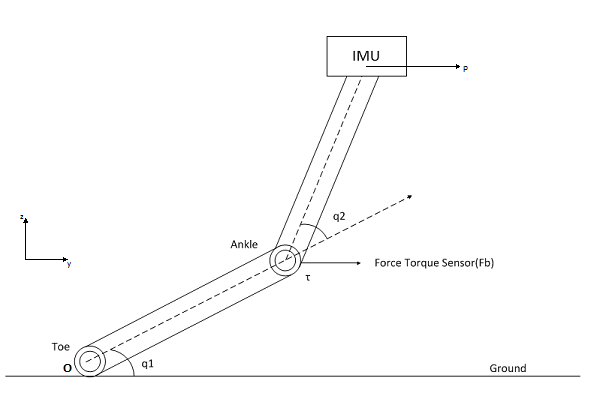
\includegraphics[scale=0.75]{Bilder/doublePendulum1.png}
	\caption{Inverted Double Pendulum}	
	\label{fig:idp}
\end{figure}
\begin{equation}
	 q = 
	\begin{pmatrix}
		q_{1}\\
		q_{2}
	\end{pmatrix}
	 \dot{q} = 
	\begin{pmatrix}
		\dot{q_{1}}\\
		\dot{q_{2}}
	\end{pmatrix}
\end{equation}

The equation of motion of the inverted double pendulum is derived by Lagrange formulation, the generalized coordinates of the system are $q_1,q_2$ which represents the angles of the joints, $\dot{q_1},\dot{q_2}$ represent the velocities of corresponding joints as shown in figure \ref{fig:idp}.
\begin{equation}
	M(q)_{2\times2}.
	\begin{pmatrix}
		\ddot{q_{1}} \\
		\ddot{q_{2}} 
	\end{pmatrix}
	+ C(q,\dot{q})_{2\times2}.
	\begin{pmatrix}
		\dot{q_{1}} \\
		\dot{q_{2}} 
	\end{pmatrix}
	+ g(q)_{2\times 1} = \tau_{2\times 1}
\end{equation}

\begin{equation}
	\label{eq:dyn_eq}
	\begin{pmatrix}
		\ddot{q_{1}} \\
		\ddot{q_{2}} 
		\end{pmatrix}
	= M(q)^{-1} \left( -C(q,\dot{q}).\dot{q} - g(q) + \tau \right )
\end{equation}

To convert the equations into ODE's, assume 
$$ x_1 = q_1, x_2 = \dot{q_1}, x_3 = q_2, x_4 = \dot{q_2}$$
substitute the above equations into \eqref{eq:dyn_eq}. The resulting non linear dynamic equation is of form

\begin{equation}
\begin{split}\label{eq:dyn_ode}
	\dot{x}  = f(x,u),	\\
	x = 
	\begin{pmatrix}
		x_1 \\
		x_2 \\
		x_3 \\
		x_4
	\end{pmatrix}
\end{split}
\end{equation}
\eqref{eq:dyn_ode} is the model prediction equations in Kalman filter. The measurement equation is,

\begin{equation}
	y= 
	\begin{pmatrix}
		q_2\\
		\dot{q_2}\\
		a_{py}\\
		a_{pz}\\
		\omega_x\\
		Fb_y\\
		Fb_z \\
	\end{pmatrix}
\end{equation}

where,
\begin{itemize}
\item
 $q_2, \dot{q_2}$- angle and velocity of ankle joint measured by encoders
\item 
$a_{py},a_{pz}$- cartesian accelerations along \emph{x and z axis} measured by IMU(Inertial Measurement Unit)
\item
$\omega_x$ - angular acceleration around \emph{x axis} measured by gyroscope
\item
$Fb_y,Fb_z$- ground reactional froces action along \emph{ y and z axis} measured by FTS(Force Torque Sensor)
\end{itemize}
The estimated states are $$q_1, \dot{q_1}$$ are the underactuated degrees of freedom of the system.
